
Una vez obtenida toda la informaci\'on posible del mu\'on a su paso por CMS, el objetivo es entrenar una red neuronal profunda tomando como entrada la informaci\'on de la traza en el tracker y la informaci\'on espacial de las se\~nales recogidas en el sistema de muones. \\
En este caso, la funci\'on de p\'erdida a minimizar ser\'a una funci\'on que dependa de la diferencia entre el $p_{T}$ de generaci\'on conocido y el $p_{T}$ que se quiere predecir, para as\'i aprender las caracter\'isticas de los muones (especialmente de aquellos que emitan cascadas) y hacer regresi\'on al momento transverso reconstruido. \\

En cuanto al software, para el entrenamiento se utiliza la librer\'ia de Python de c\'odigo abierto Keras~\cite{chollet2015keras}, que se caracteriza principalmente por ofrecer sencillez de uso para el usuario, y la red se ejecuta sobre TensorFlow~\cite{tensorflow2015-whitepaper}.


\subsection{Variables de entrenamiento}\label{sec:variables}

Las variables utilizadas para el entrenamiento se dividen en dos categor\'ias seg\'un su naturaleza:

\begin{itemize}
\item Caracter\'sticas de la traza interna reconstruida en el tracker: $p_{T}$, $\eta$, $\phi$, carga.
\item Informaci\'on del conjunto de segmentos recogidos en cada estaci\'on de DTs y CSCs: n\'umero total de segmentos en la estaci\'on, media espacial en x, y, z, desviaci\'on est\'andard en x, y, z, asimetr\'ia en x, y, z, kurtosis en x, y, z.
\end{itemize}

En la Figura~\ref{fig:train_vars} se muestran las distribuciones de las variables utilizadas en el entrenamiento provenientes de la traza del tracker y de las estaciones de las DTs.

\begin{figure}
\centering
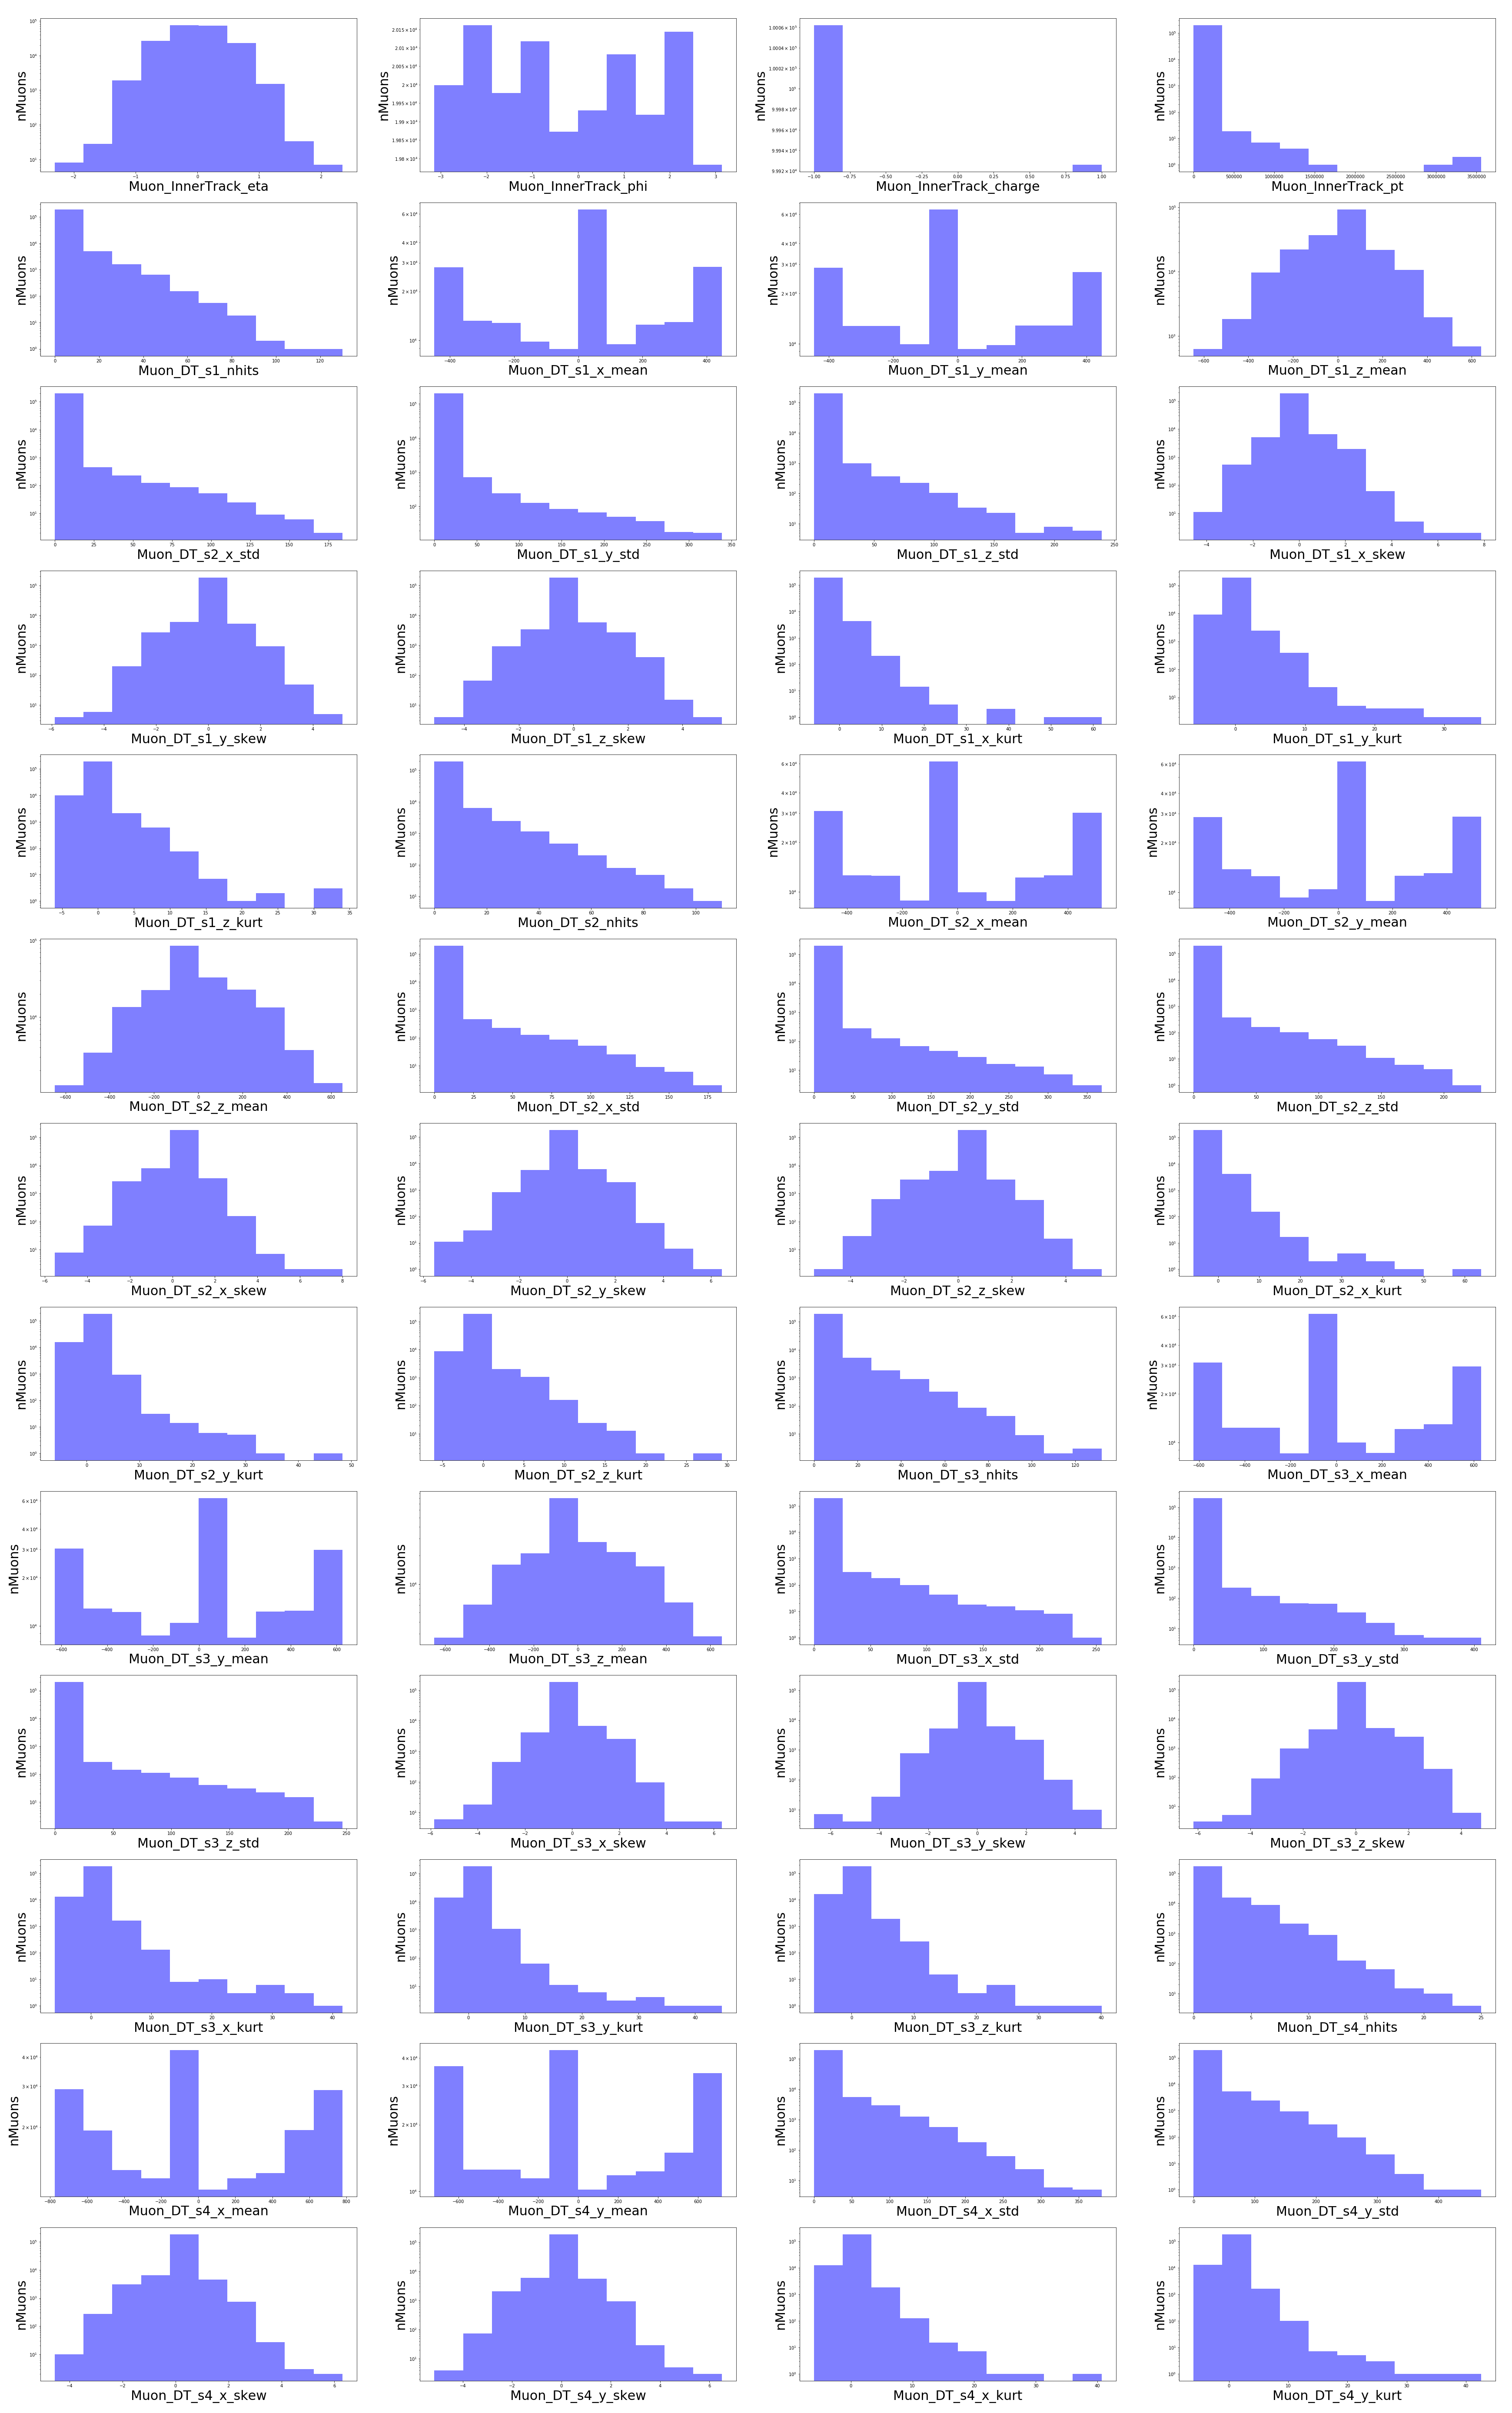
\includegraphics[width=1.0\textwidth]{figures/Training_vars_2.png}
\caption{Distribuciones de las variables de entrenamiento}
\label{fig:train_vars}        
\end{figure}


\subsection{Conjunto de datos y arquitectura de la red}\label{sec:arch}

El conjunto de datos, compuesto por un total de 195777 muones, se ha dividido en un 80\% para el entrenamiento del modelo (del que un 10\% ser\'a usado como conjunto de datos de validaci\'on), mientras que un 20\% es utilizado para el testeo del mismo. \\

En cuanto al tipo de red utilizada, se ha entrenado una red de tipo \textit{fully-conected}, donde todos los nodos de cada capa est\'an conectados con los nodos de las capas contiguas, con la siguiente arquitectura:


\begin{itemize}

\item Activaci\'on: Para las capas 1-9 se utliza la funci\'on de activaci\'on ReLu~\cite{agarap2018deep}, ya que es una de las funciones de activaci\'on m\'as apropiadas para problemas de aprendizaje profundo por tener siempre derivada 1 y as\'i evitar el problema del \textit{vanishing gradient}~\cite{Hochreiter:91}. En la \'ultima capa 10 se utiliza una funci\'on de activaci\'on lineal para hacer regresi\'on al $p_{T}$.

\item Como optimizador se usa Adam (del ingl\'es \textit{Adaptative Moment estimation}), que combina el Gradient Descent con momento con el Gradient descent con RMSprop, con tasa de aprendizaje = 0.0005 y el resto de hiperpar\'ametros los recomendados por el art\'iculo original de Adam~\cite{Kingma2015AdamAM}.

\item Funci\'on de p\'erdida: MSE (del ingl\'es \textit{Mean Squared Error}).

\item \'Epocas de entrenamiento: 1000.

\item Descenso del gradiente: para agilizar el apredizaje se hace uso de la t\'ecnica del \textit{mini-batch gradient descent}~\cite{perrone2019optimal}, que consiste en dividir el conjunto de datos de entrenamiento en fragmentos peque\~nos denominados \textit{mini-batches}, de manera que los par\'ametros de la red se van actualizando para cada fragmento sin tener que recorrer toda la muestra, mejorando considerablemente la velocidad en el entrenamiento y consiguiendo una buena convergencia. El tama\~no del mini-batch elegido ha sido de 2000 muones.

\item Para regularizar se utiliza la t\'ecnica de \textit{Early stopping} en la p\'erdida del conjunto de datos de validaci\'on, con una paciencia de 50 \'epocas. De esta manera, para cada \'epoca se obtiene el valor del MSE en el conjunto de datos de validaci\'on (que no se utilizan para entrenar). Si el MSE no mejora despu\'es de 50 \'epocas se guarda el modelo encontrado con menor MSE en validaci\'on y se detiene el entrenamiento para evitar as\'i que el modelo sobreentrene. 

\end{itemize}

El valor de los hiperpar\'ametros se ha tomado tras probar distintas configuraciones aleatorias de los mismos (b\'usqueda de tipo cuadr\'icula), y se ha elegido aquella que proporciona un MSE menor en el conjunto de datos de testeo.
  

\subsection{Resultados del entrenamiento}\label{sec:trainresults}

En la Figura~\ref{fig:model_loss} se muestra la el valor de la p\'erdida MSE en funci\'on de la \'epoca de entrenamiento. \\
El mejor modelo de obtiene despu\'es de 184 \'epocas, con un valor de p\'erdida para el conjunto de datos de entrenamiento de 49605.3, para el conjunto de datos de validaci\'on de 50399.8, y para el conjunto de datos de testeo de 53731.6.  \\

\begin{figure}[h]
\centering
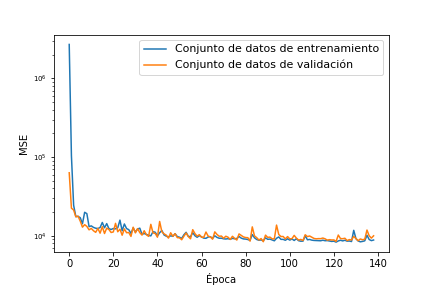
\includegraphics[width=0.6\textwidth]{figures/model_loss.png}
\caption{Valor del MSE en funci\'on de la \'epoca de entrenamiento para el conjunto de datos de entrenamiento (en azul) y para el conjunto de datos de validaci\'on (en naranja).}
\label{fig:model_loss}        
\end{figure}


En la Figura~\ref{fig:R_predicted} se comparan la distribuciones de la resoluci\'on R, definida en \eqref{eq:R}, calculadas sobre el conjunto de datos de testeo a partir del $p_{T}$ que da el algoritmo TuneP y a partir del $p_{T}$ que predice la red neuronal respectivamente.

\begin{figure}[h]
\centering
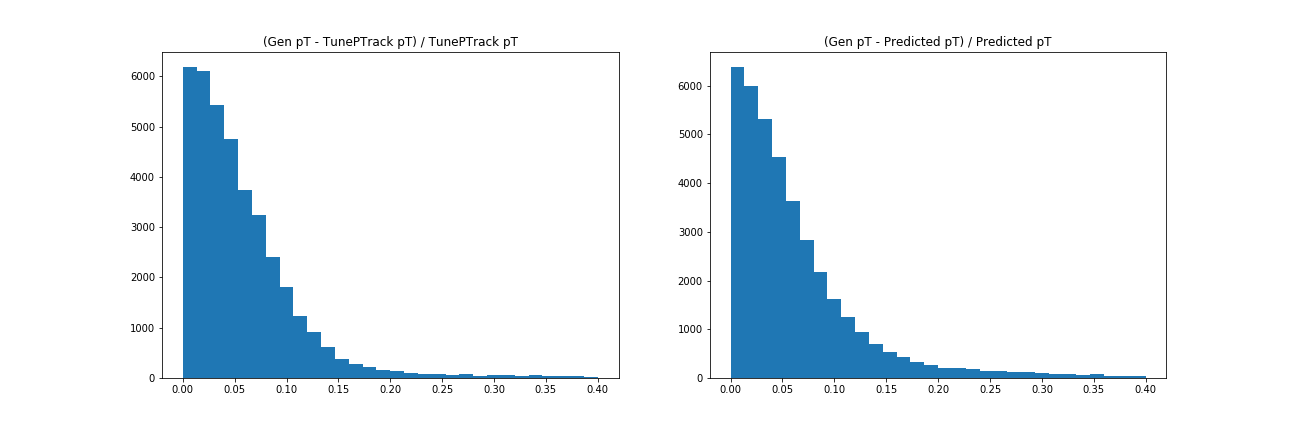
\includegraphics[width=1.0\textwidth]{figures/R_predicted.png}
\caption{Distribuci\'on de la resoluci\'on R dada por \eqref{eq:R} sobre el conjunto de datos de testeo. Izquierda: tomando el $p_{T}$ que da el algoritmo TuneP. Derecha: tomando el $p_{T}$ predicho por el modelo de regresi\'on al $p_{T}$.}
\label{fig:R_predicted}        
\end{figure}

